\documentclass{beamer}
\usepackage{beamerthemesplit}
\usepackage{wrapfig}
\usetheme{SPbGU}
\usepackage{pdfpages}
\usepackage{amsmath}
\usepackage{cmap} 
\usepackage[T2A]{fontenc} 
\usepackage[utf8]{inputenc}
\usepackage[english,russian]{babel}
\usepackage{indentfirst}
\usepackage{amsmath}
\usepackage{tikz}
\usepackage{multirow}
\usepackage[noend]{algpseudocode}
\usepackage{algorithm}
\usepackage{algorithmicx}
\usetikzlibrary{shapes,arrows}
\usepackage{fancyvrb}
\usepackage{tikz}
\usepackage{pgfplots}
\usetikzlibrary{calc}
\usetikzlibrary{shapes,arrows}
\usetikzlibrary{arrows,automata,arrows.meta}
\usetikzlibrary{positioning}
\usepackage[labelformat=empty]{caption}
\usepackage[labelformat=empty]{subcaption}
\beamertemplatenavigationsymbolsempty
\usepackage{multirow}
\usepackage{verbatim}
\usepackage{array}
\usepackage{graphicx}
\usepackage{multirow} 
\usepackage{appendixnumberbeamer}
\usepackage{fancyvrb}
\usepackage[misc,geometry]{ifsym} 
\usepackage{multicol}
\newcolumntype{P}[1]{>{\centering\arraybackslash}p{#1}}
\newcommand{\tikzmark}[1]{\tikz[overlay,remember picture] \node (#1) {};}
\def\Put(#1,#2)#3{\leavevmode\makebox(0,0){\put(#1,#2){#3}}}
\newcommand{\ltz}{$< 1$}
\tikzset{
    state/.style={
           rectangle,
           rounded corners,
           draw=gray, very thick,
           minimum height=2em,
           inner sep=2pt,
           text centered,
           },}

\title[]{Комбинирование нейронных сетей и синтаксического анализа для предсказания вторичной структуры генетических цепочек}

\institute[СПбГУ]{
Санкт-Петербургский государственный университет}

\author[Лунина Полина]{Лунина Полина Сергеевна \\
  \and  
    {\bfseries Научный руководитель:} Григорьев С.В. \\
	\and
	{\bfseries Рецензент:} Малыгина Т.С.}

\date{9 июня 2021г.}

\begin{document}
{
\begin{frame}[fragile]
  \begin{tabular}{p{2.0cm} p{7.5cm} p{1cm}}
   \begin{center}
      
\includegraphics[height=1.5cm]{pics/jetbrainsResearch.pdf}
    \end{center}
    &
    \begin{center}
      
\includegraphics[height=1.5cm]{pics/YC_logo.pdf}
    \end{center}
    &
    \begin{center}
      
\includegraphics[height=1.5cm]{pics/SPbGU_Logo.png}
    \end{center}
  \end{tabular}
  \titlepage
\end{frame}
}

\begin{frame}{Введение}
\textbf{Геномные последовательности}
\begin{itemize}
    \item РНК
    \item ДНК
    \item Белки
\end{itemize}

\vspace{3mm} 

\textbf{Уровни молекулярной организации}
\begin{itemize}
    \item Первичная структура (линейная)
    \item Вторичная структура (пространственная)
\end{itemize}

\vspace{3mm} 

\textbf{Задачи}
\begin{itemize}
    \item Распознавание последовательностей
    \item Классификация организмов
    \item Предсказание вторичных структур
    \item ...
\end{itemize}
\end{frame}

\begin{frame}{Вторичная структура РНК}
\begin{tabular}{cl}  
    \parbox{0.6\linewidth}{
        \textbf{Значение}
        \begin{itemize}
            \item Транскрипция, трансляция
            \item Филогенетика, таксономия
        \end{itemize}
        
        \vspace{3mm}  
        
        \onslide<2>{
        \textbf{Методы предсказания}  
        \begin{itemize}
            \item Лабораторные
            \item Сравнительные
            \item Вычислительные
            \begin{itemize}
                \item Минимизация свободной \linebreak энергии
                \item Стохастические модели и грамматики
                \item Машинное обучение
                \item ...
            \end{itemize}
        \end{itemize}}}
    & \begin{tabular}{l}
        \hspace{-1.8cm}
        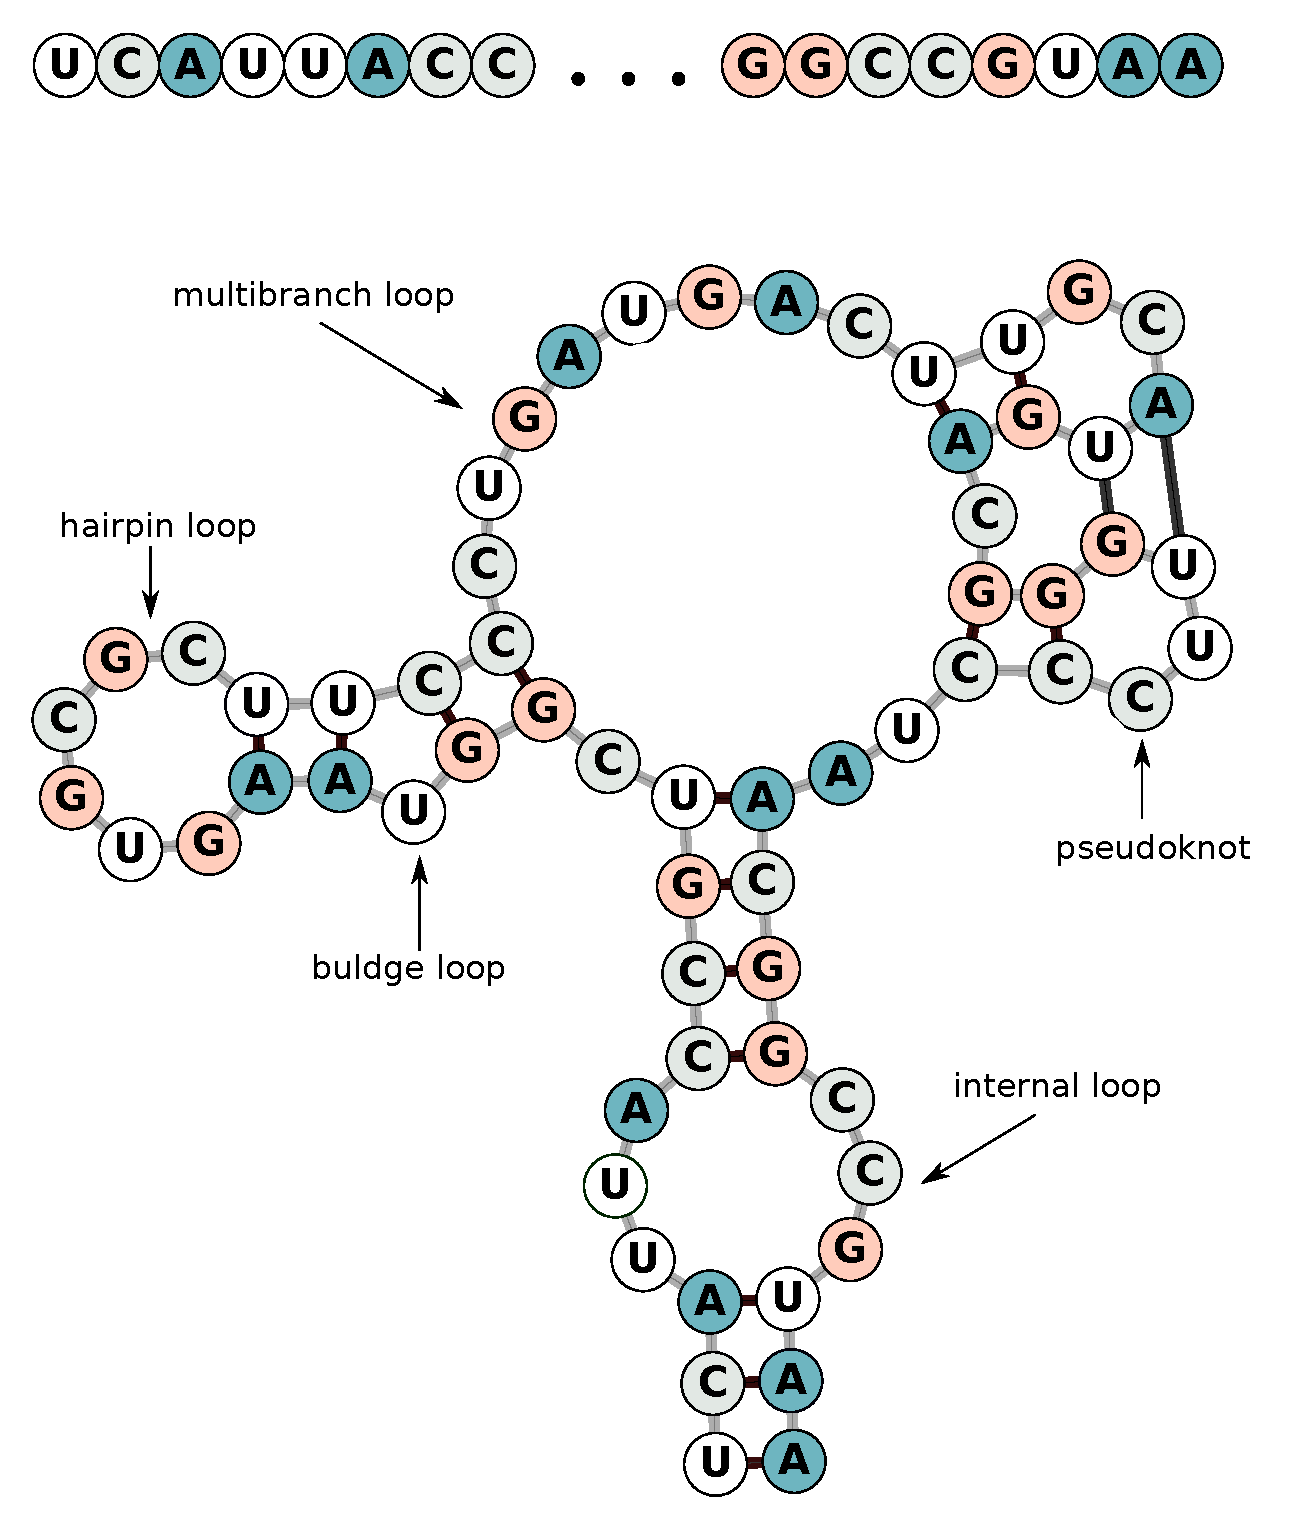
\includegraphics[width=6.0cm]{pics/rna.pdf}
    \end{tabular}  \\
\end{tabular}
\end{frame}

\begin{frame}{Вторичная структура РНК}
\begin{tabular}{cl}  
    \parbox{0.6\linewidth}{
        \textbf{Проблемы}  
        \begin{itemize}
            \item Сложность формализации
            \item Предсказание псевдоузлов
            \item Вариативность элементов
            \item Зашумленность данных
        \end{itemize}
        
        \vspace{6mm} 

        \onslide<4>{        
        \textbf{Наше решение}
        \begin{itemize}
            \item Формальная грамматика для описания базовых законов
            \item Нейронная сеть для синтеза вторичной структуры
        \end{itemize}}}
    & \begin{tabular}{l}
        \hspace{-1.8cm}
        \begin{overprint}
        \onslide<1,3,4>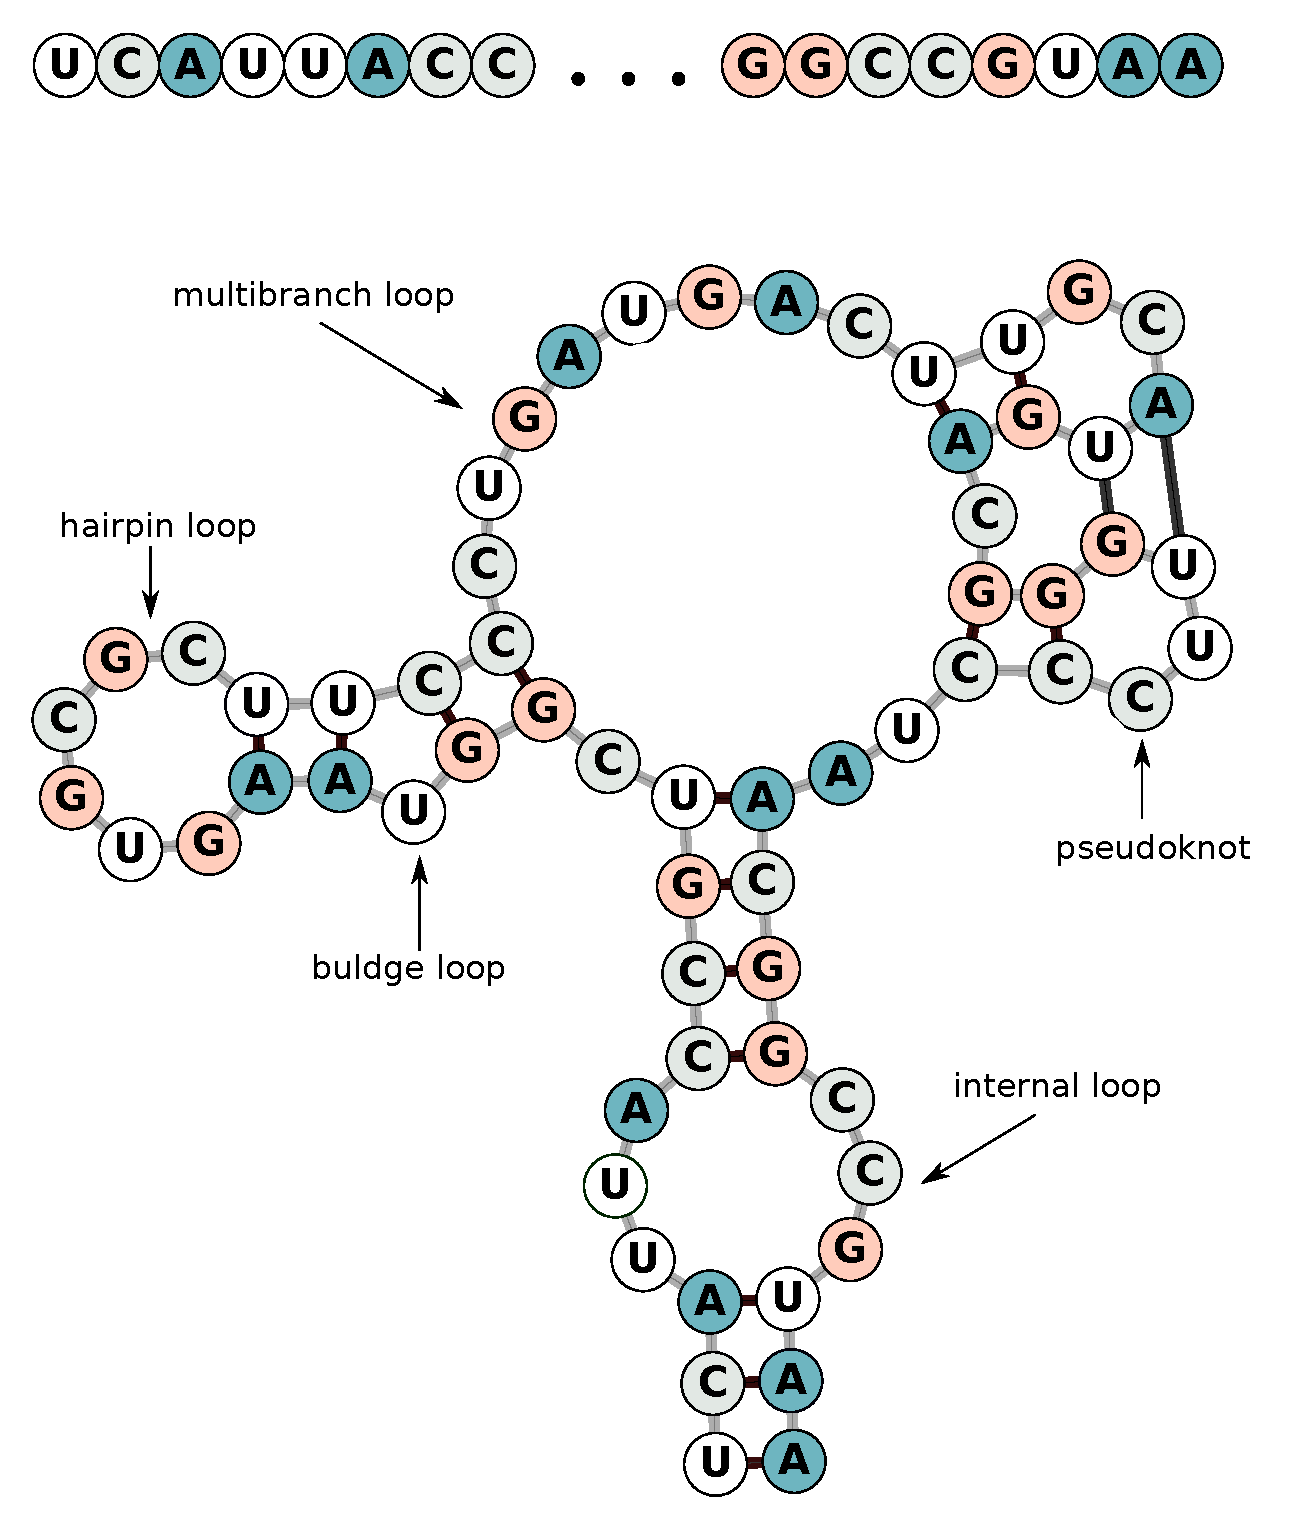
\includegraphics[width=6.0cm]{pics/rna.pdf}
        \onslide<2>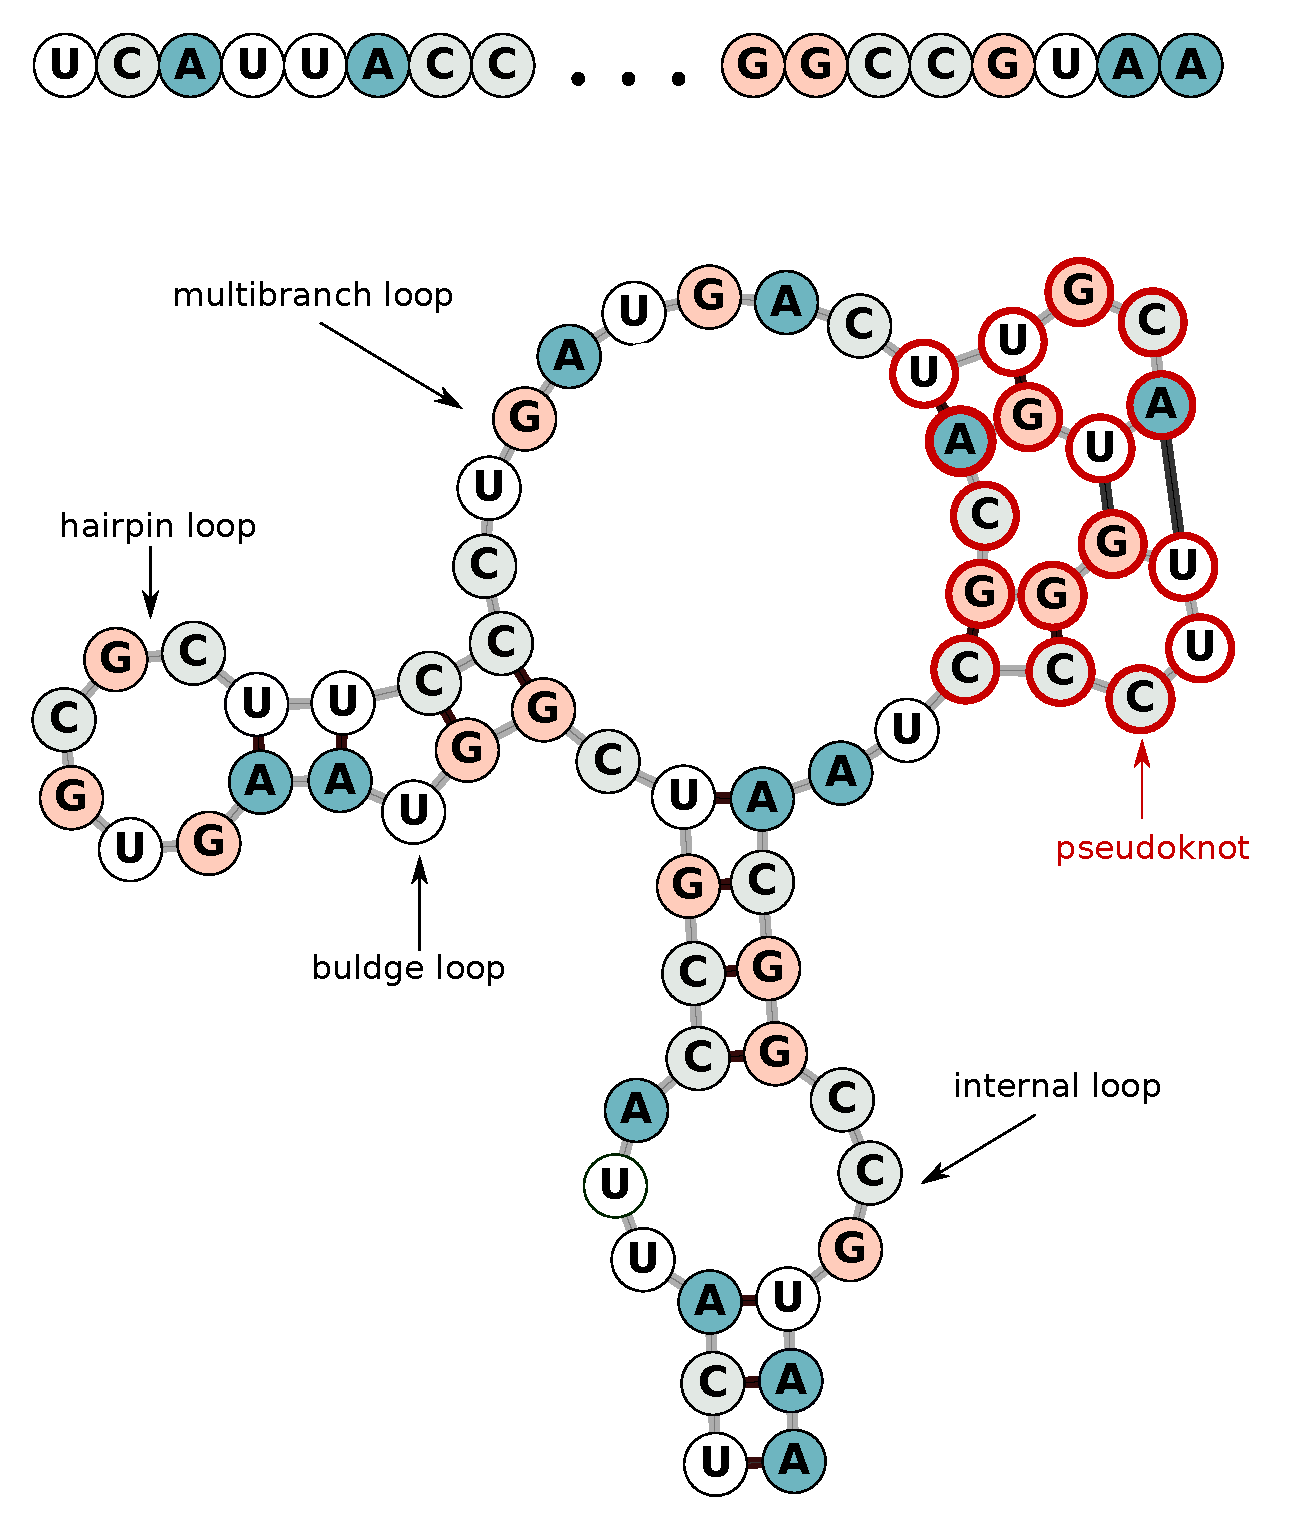
\includegraphics[width=6.0cm]{pics/rna_2.pdf}
        \end{overprint}
    \end{tabular}  \\
\end{tabular}
\end{frame}

\begin{frame}{Постановка задачи}
\textbf{Цель} --- исследование возможности применения подхода, основанного на комбинировании нейронных сетей и синтаксического анализа, к задаче предсказания вторичной структуры молекулы РНК

\vspace{6mm}

\textbf{Задачи}
\begin{itemize}
    \item Разработка архитектуры решения, конкретизирующей форматы данных, используемые грамматики и нейронные сети
    \item Проведение экспериментальных исследований, сравнение с аналогами
\end{itemize}
\end{frame}

\begin{frame}{Архитектура решения}
\vspace{0.3cm}\hspace{0.2cm}
\scriptsize
  \begin{tikzpicture}[->,>=triangle 45]
  \node[state,
        align=left,
        text width = 4.0cm] (grm)
   {
   \textbf{Формальная грамматика}\\
   Описывает базовые элементы вторичной структуры
   };

  \node[state,
        below = 0.8cm of grm,
        align = left,
        text width = 4.0cm] (sqs)
   {
   \textbf{Последовательности РНК}\\ 
   Строки над алфавитом $\{A, C, G, U\}$
   };

  \node[state,
        below right = -1.1cm and 2cm of grm,
        align = left,
        double,
        double distance=1.5mm,
        inner sep=1.5mm,
        minimum height = 3cm,
        text width = 4.6cm](parser)
  {
  \textbf{Синтаксический анализатор}\\
  Осуществляет поиск базовых \linebreak элементов вторичной структуры \linebreak в последовательностях РНК
  };

  \node[state,
        below = 1.2cm of parser,
        align = left,
        text width = 4.0cm](mtrx)
  {
  \textbf{Матрицы разбора}\\
  Извлеченная синтаксическим анализатором информация
  };

  \node[state,
        below = 1.2cm of sqs,
        minimum height = 3cm,
        align = left,
        double,
        double distance=1.5mm,
        inner sep=1.5mm,
        text width = 4.6cm](NN)
  {
  \textbf{Нейронная сеть}\\
  Обрабатывает матрицы разбора \linebreak и предсказывает вторичную \linebreak структуру последовательностей
  };
  
    \node[state,
        below = 3.1cm of parser,
        align = left,
        text width = 4.0cm](ss)
  {
  \textbf{Вторичные структуры}\\
  Результат предсказания \linebreak нейронной сети
  };

 \path (grm.east) edge (4,0)
   (sqs.east) edge (4,-1.9)
   (6.55,-2.6) edge (mtrx)
   (mtrx.west) edge (2.6,-4.25)
   (2.6,-6.15) edge (ss.west)
   ;
\end{tikzpicture}

\tikzmark{zzz}{}

\onslide<2>{
\tikz[overlay,remember picture]{\draw[draw=gray, very thick,fill=red, fill opacity=0.1, rounded corners] ($ (zzz) + (0.82,7.67)$) rectangle ($ (zzz) + (4.97,6.6)$);}
\tikz[overlay,remember picture]{\draw[draw=gray,very thick,fill=red, fill opacity=0.1, rounded corners] ($ (zzz) + (0.82,5.77)$) rectangle ($ (zzz) + (4.97,4.7)$);}}

\onslide<3>{
\tikz[overlay,remember picture]{\draw[draw=gray,very thick,fill=red, fill opacity=0.1, rounded corners=7pt] ($ (zzz) + (6.9,7.77)$) rectangle ($ (zzz) + (12.0,4.57)$);}
\tikz[overlay,remember picture]{\draw[draw=gray,very thick,fill=red, fill opacity=0.1, rounded corners] ($ (zzz) + (7.4,3.44)$) rectangle ($ (zzz) + (11.55,2.37)$);}}

\onslide<4>{
\tikz[overlay,remember picture]{\draw[draw=gray,very thick,fill=red, fill opacity=0.1, rounded corners=7pt] ($ (zzz) + (0.35,3.57)$) rectangle ($ (zzz) + (5.45,0.37)$);}
\tikz[overlay,remember picture]{\draw[draw=gray,very thick,fill=red, fill opacity=0.1, rounded corners] ($ (zzz) + (7.37,1.54)$) rectangle ($ (zzz) + (11.52,0.47)$);}}

\end{frame}

\begin{frame}[fragile]{Формальная грамматика}
\begin{itemize}
    \item Вторичная структура как рекурсивная композиция базовых элементов --- шпилек (stem-loop)
    \item КС грамматика для описания общего вида шпильки
    \item Ограничения: размер петли (1-20), высота (от 3), канонические пары (A-U, C-G)
\end{itemize}

\vspace{6mm}

\begin{figure}
    \centering
    \begin{subfigure}{.47\textwidth}
        \centering
        \begin{overprint}
            \onslide<1,7,8>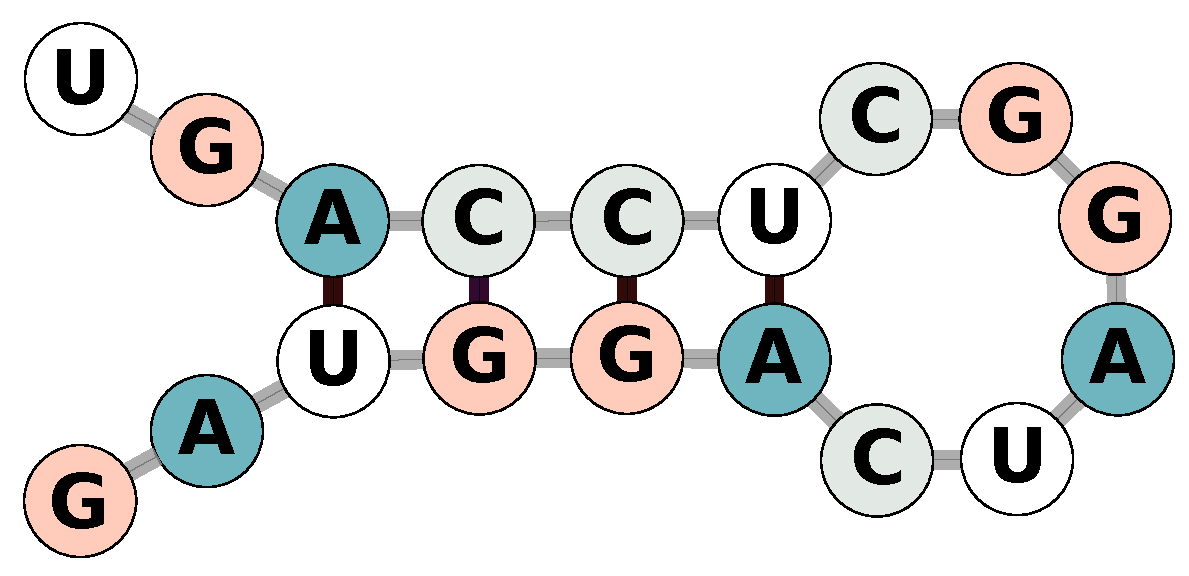
\includegraphics[width=4.5cm]{pics/stem.pdf}
            \onslide<2>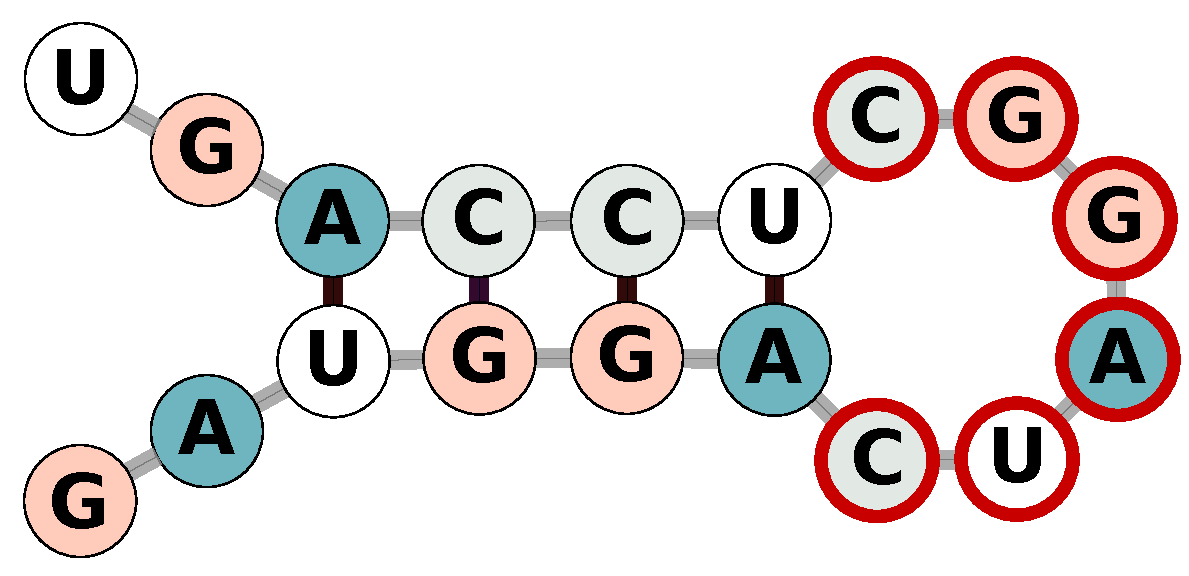
\includegraphics[width=4.5cm]{pics/stem_2.pdf}
            \onslide<3>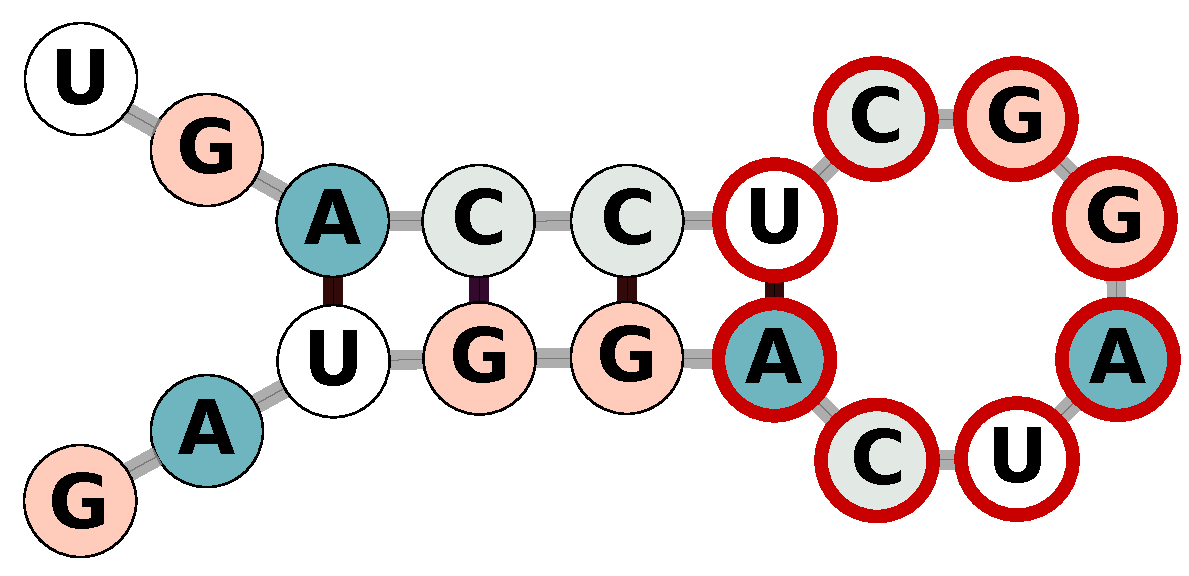
\includegraphics[width=4.5cm]{pics/stem_3.pdf}
            \onslide<4>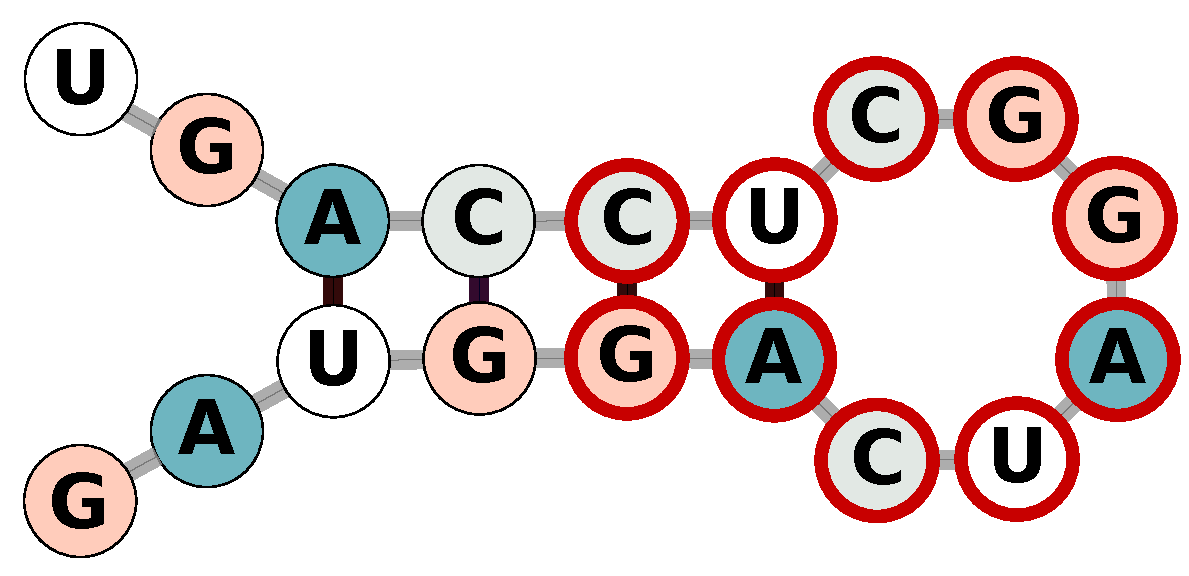
\includegraphics[width=4.5cm]{pics/stem_4.pdf}
            \onslide<5>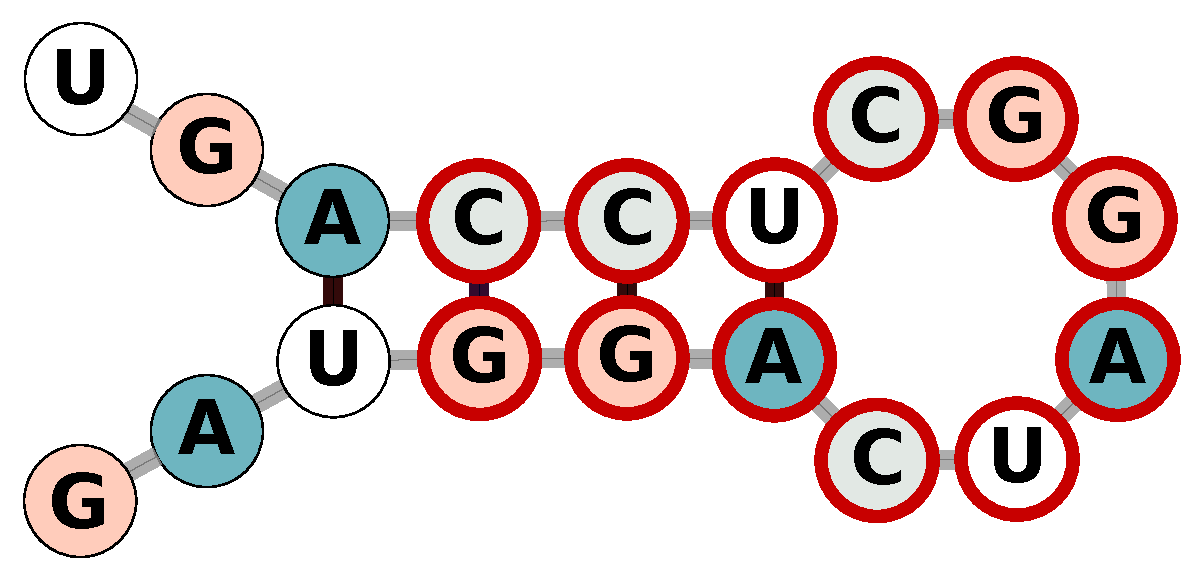
\includegraphics[width=4.5cm]{pics/stem_5.pdf}
            \onslide<6>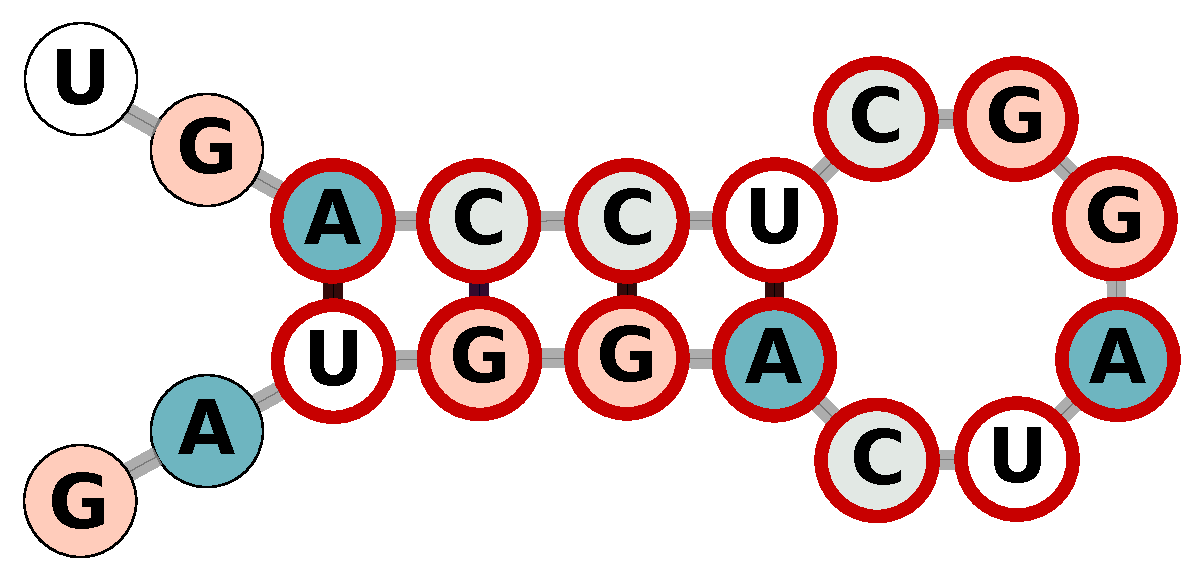
\includegraphics[width=4.5cm]{pics/stem_6.pdf}
        \end{overprint}
    \end{subfigure}%
    \begin{subfigure}{.53\textwidth}
    \centering
    \footnotesize
\begin{Verbatim}
start: stem3<s0>
s0: loop | loop stem3<s0> s0
loop: nucl*[1..20]
nucl: A | U | C | G
stem1<s>: A s U | G s C | U s A | C s G
stem2<s>: stem1<stem1<s>>
stem3<s>: 
      stem1<stem2<s>>
    | A stem3<s> U
    | U stem3<s> A
    | C stem3<s> G
    | G stem3<s> C
\end{Verbatim}
    \end{subfigure}
\end{figure}

{\tikz[overlay,remember picture]{\draw[draw=black,thick,fill opacity=0.2] ($ (5.55,4.75)$) rectangle ($ (12.25,0.05)$);}}

\onslide<2>{{\tikz[overlay,remember picture]{\draw[fill=red, fill opacity=0.1] ($ (5.55,4.45)$) rectangle ($ (8.85,3.7)$);}}}

\onslide<3>{{\tikz[overlay,remember picture]{\draw[fill=red, fill opacity=0.1] ($ (5.55,4.15)$) rectangle ($ (12.25,3.75)$);}}}

\onslide<4>{{\tikz[overlay,remember picture]{\draw[fill=red, fill opacity=0.1] ($ (5.55,4.25)$) rectangle ($ (9.85,3.85)$);}}}

\onslide<5>{{\tikz[overlay,remember picture]{\draw[fill=red, fill opacity=0.1] ($ (5.55,4.3)$) rectangle ($ (9.15,3.6)$);}}}

\onslide<6>{{\tikz[overlay,remember picture]{\draw[fill=red, fill opacity=0.1] ($ (5.55,4.8)$) rectangle ($ (9.15,2.45)$);}}}

\onslide<7>{{\tikz[overlay,remember picture]{\draw[fill=red, fill opacity=0.1] ($ (5.55,7.6)$) rectangle ($ (10.35,6.85)$);}}}

\onslide<8>{}
\end{frame}

\begin{frame}{Синтаксический анализатор}
\begin{itemize}
    \item Задача поиска всех возможных шпилек в последовательности
    \item Результат работы --- матрица разбора \linebreak $M_p(seq)$: $M_p[i,j]=1 \iff seq[i..j]$ выводима в грамматике
    \item Шпильке высоты $n \geq 3$ соответствует столбик из $n - 2$ единиц
\end{itemize}

\vspace{3mm}

\centering
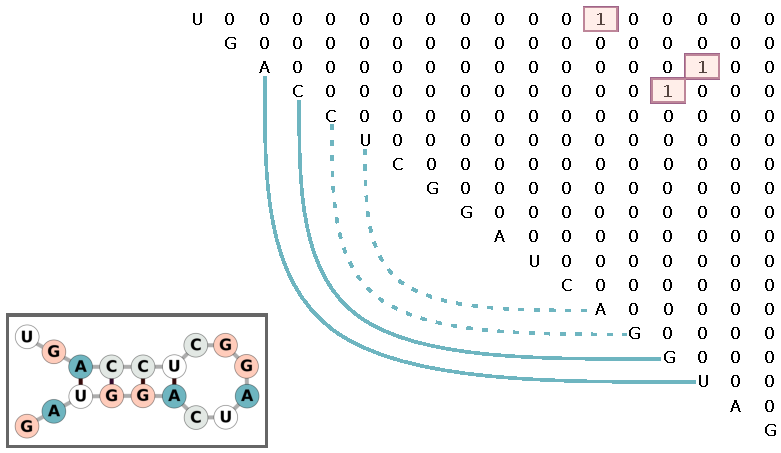
\includegraphics[width=.79\textwidth]{pics/matrix.pdf}
\end{frame}

\begin{frame}{Синтаксический анализатор}
\begin{itemize}
    \item Псевдоузлы не выводимы в КС грамматике
    \item Шпильки, из которых они состоят, выводимы по отдельности
\end{itemize}
\hspace{0.15cm} $\Rightarrow$ Наш подход позволяет учитывать псевдоузлы

\vspace{3mm}

\centering
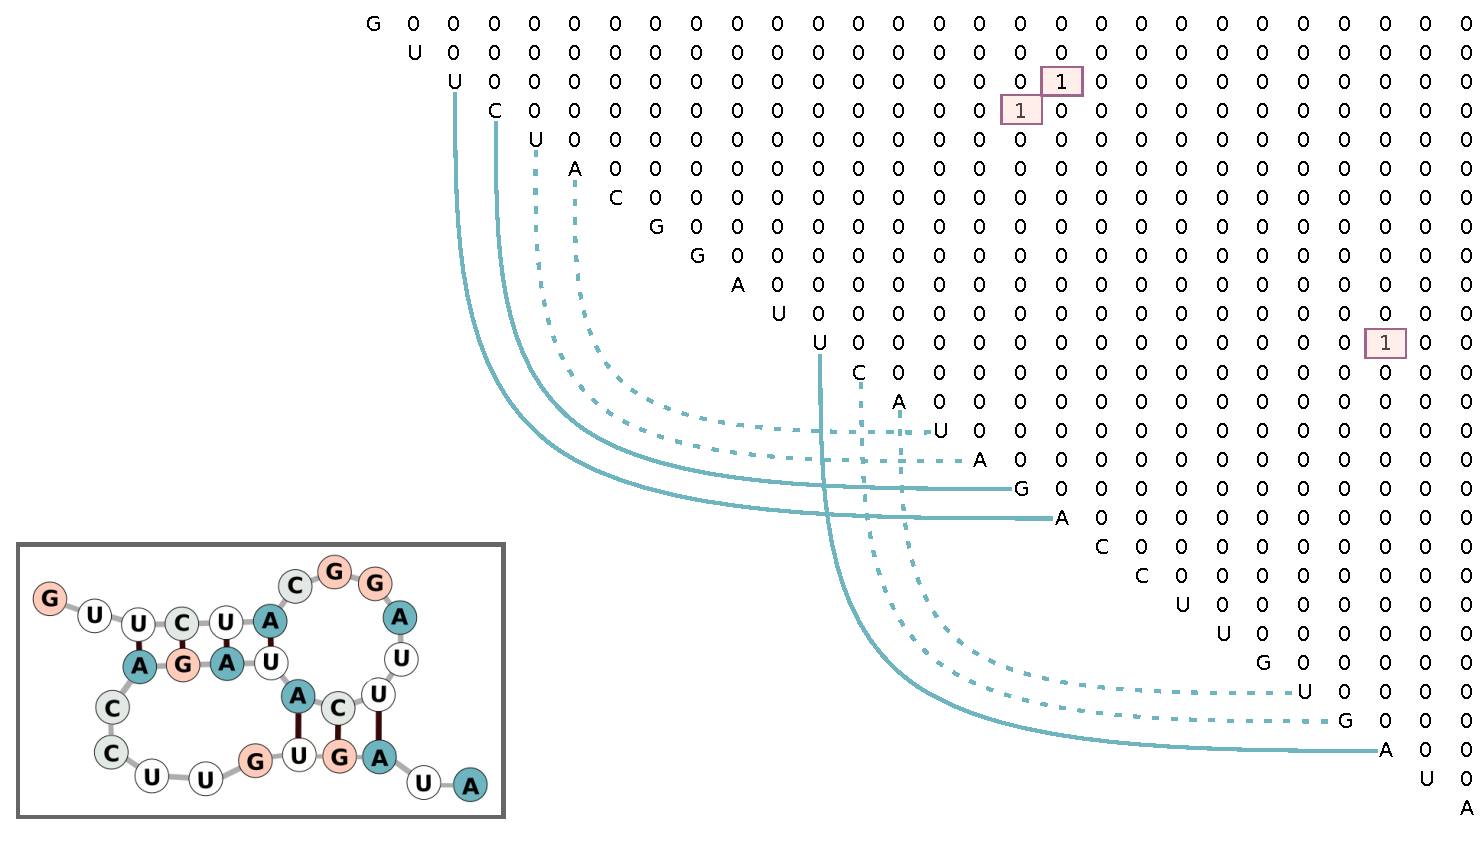
\includegraphics[width=.85\textwidth]{pics/matrix2.pdf}
\end{frame}

\begin{frame}{Нейронная сеть}
\begin{itemize}
    \item Парсер находит все возможные шпильки $\Rightarrow$ избыточность $M_p$
    \item В грамматике есть ограничения $\Rightarrow$ недостаточность $M_p$
    \item Решение --- обработка матриц разбора нейронной сетью
    \item Эталон --- матрица контактов реальной вторичной структуры $M_c(seq)$: $M_c[i,j]=1 \iff seq[i]$ и $seq[j]$ образуют контакт
\end{itemize}

\vspace{3mm}

\captionsetup[subfigure]{justification=centering}
\setlength{\fboxsep}{0pt}
\begin{figure}[h]
    \centering
    \begin{subfigure}{.33\textwidth}
        \centering
        \vspace{-3.5mm}
        \begin{overprint}
        \onslide<1>\fbox{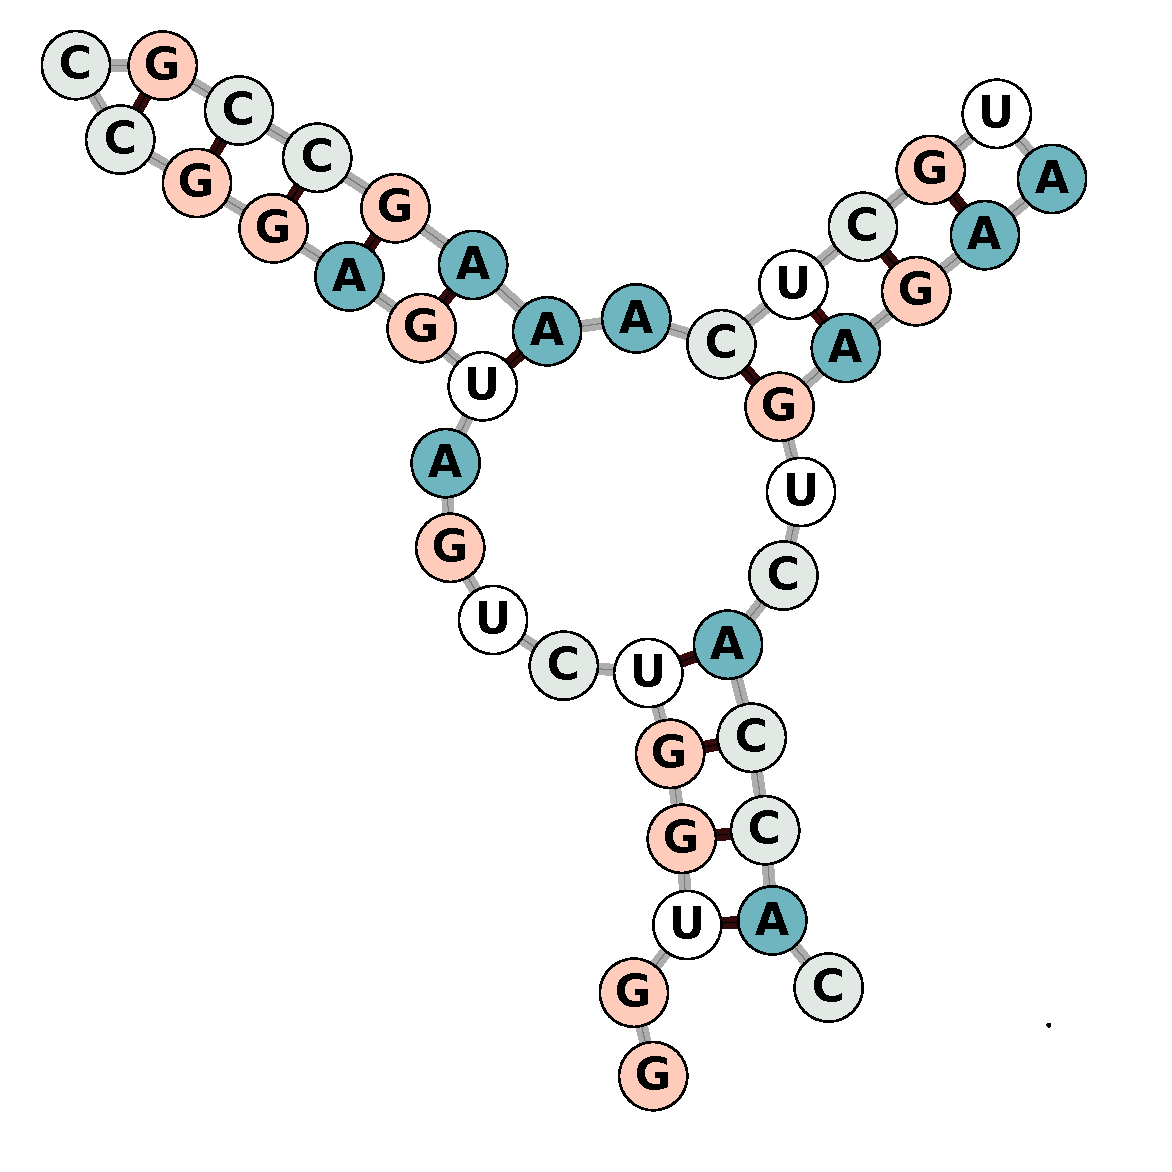
\includegraphics[width=.95\linewidth]{pics/struct.pdf}}
        \onslide<2>\fbox{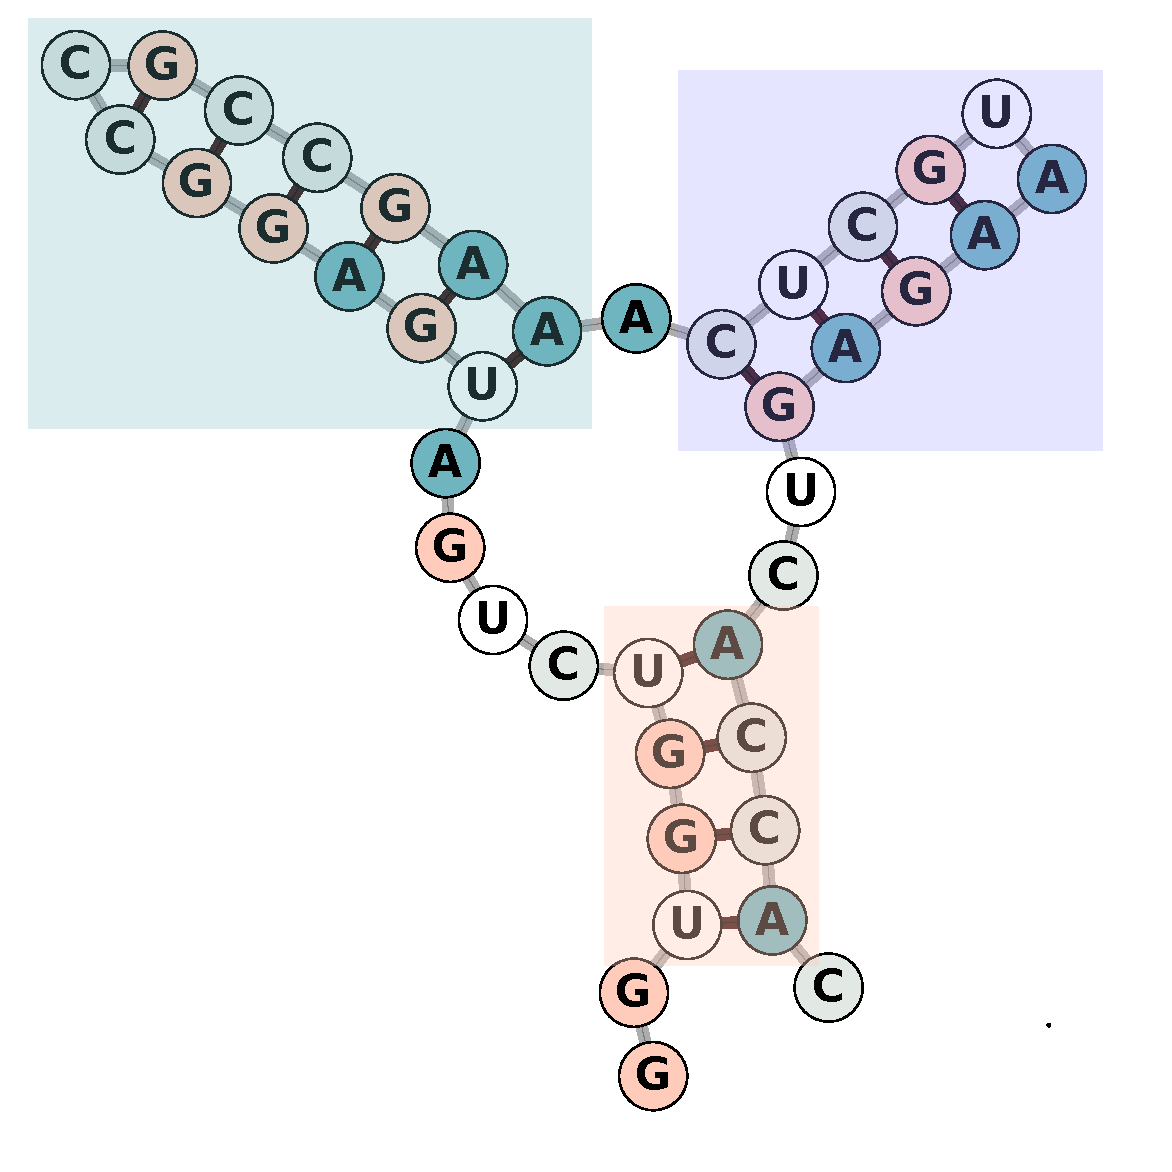
\includegraphics[width=.95\linewidth]{pics/struct2.pdf}}
        \end{overprint}
        \caption{Вторичная структура}
    \end{subfigure}%
    \begin{subfigure}{.33\textwidth}
          \centering
          \begin{overprint}
          \onslide<1>\fbox{
\includegraphics[width=.95\linewidth]{pics/out.png}}
          \onslide<2>\fbox{
\includegraphics[width=.95\linewidth]{pics/out_2.png}}
          \end{overprint}
          \caption{Эталонное изображение (матрица контактов)}
    \end{subfigure}%
    \begin{subfigure}{.33\textwidth}
          \centering
          \begin{overprint}
          \onslide<1>\fbox{
\includegraphics[width=.95\linewidth]{pics/in.png}}
          \onslide<2>\fbox{
\includegraphics[width=.95\linewidth]{pics/in_2.png}}
          \end{overprint}
          \caption{Входное изображение (матрица разбора)}
    \end{subfigure}%
\end{figure}
\end{frame}

\begin{frame}{Нейронная сеть}
\begin{itemize}
    \item Параллельная остаточная архитектура
    \item Dropout и L2-регуляризация для снижения переобучения
\end{itemize}

\vspace{3mm}

\centering
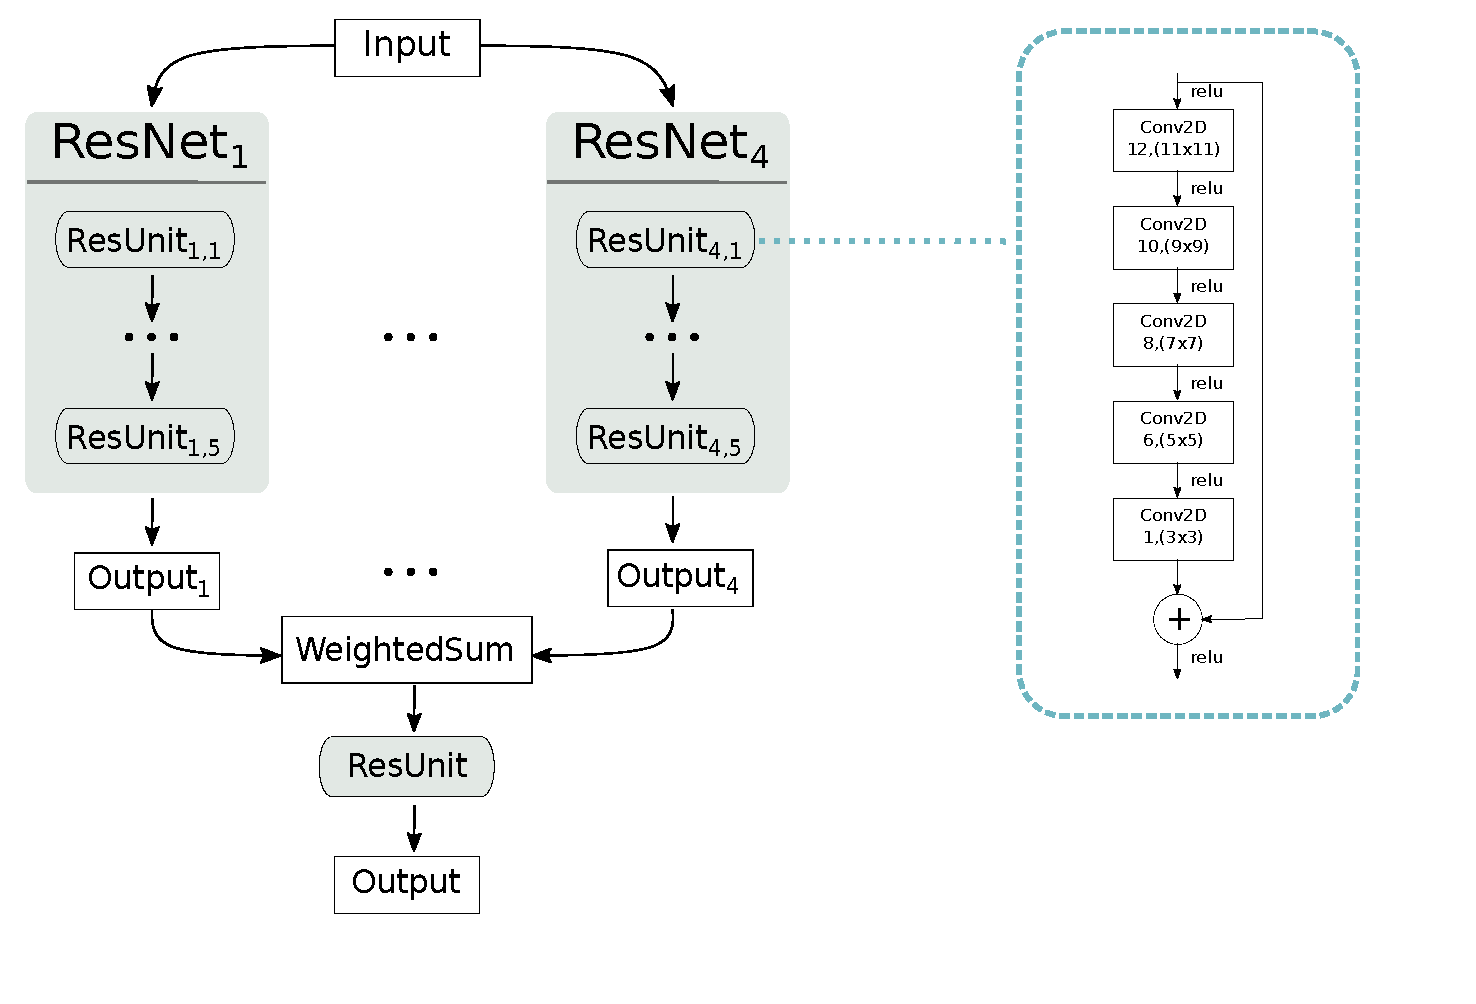
\includegraphics[width=10cm]{pics/nn.pdf}
\end{frame}

\begin{frame}{Эксперименты}
\textbf{Задача --- } предсказание вторичных структур для цепочек РНК с имеющимися достоверными эталонными данными 

\vspace{3mm}

\textbf{Данные}
\begin{itemize}
    \item База RNAstrand (последовательности + вторичные структуры)
    \item 800 последовательностей длины до 100 (74 с псевдоузлами)
    \item Data augmentation --- отражение относительно побочной диагонали
\end{itemize}

\vspace{3mm}

\textbf{Технологии}
\begin{itemize}
    \item Синтаксический анализ: платформа YaccConstructor
    \item Нейронные сети: библиотека Keras и фреймворк Tensorflow 
\end{itemize}

\vspace{3mm}

\centering
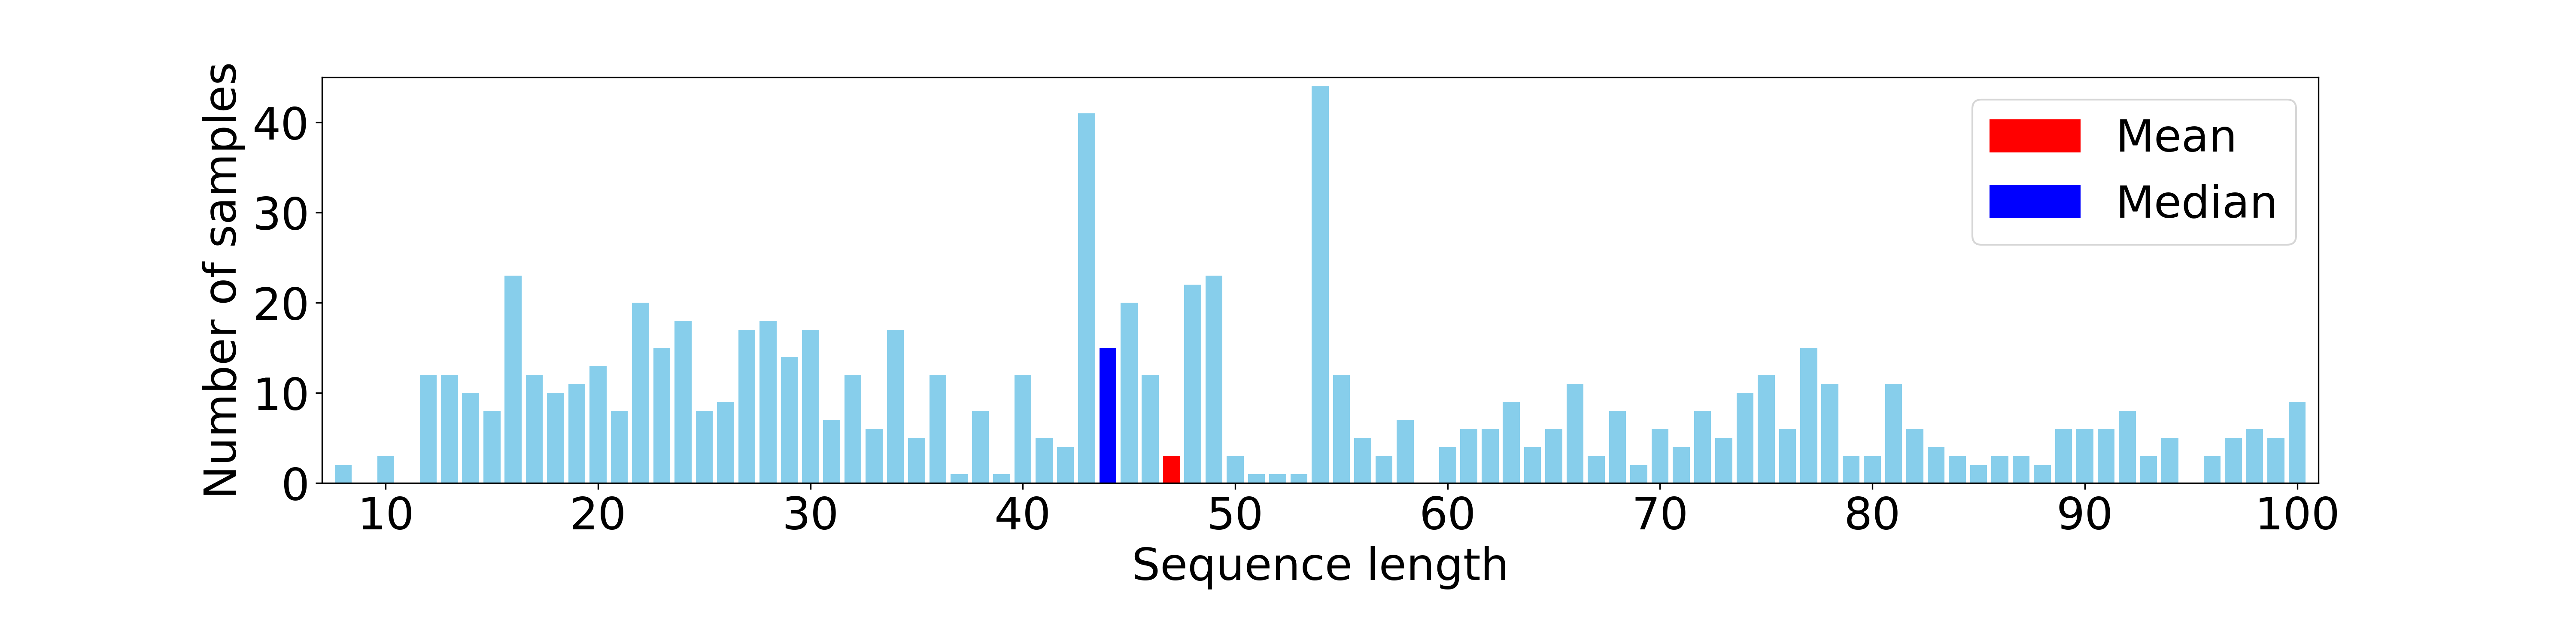
\includegraphics[width=\textwidth]{pics/plot_distr.png}
\end{frame}

\begin{frame}{Эксперименты}
\textbf{Аналоги}
\begin{itemize}
    \item HotKnots --- MFE + эвристический алгоритм 
    \item SPOT-RNA --- машинное обучение
    \item PknotsRG --- MFE + Turner energy rules 
    \item RNAstructure --- MFE + динамическое программирование 
    \item Ipknot --- MEA + целочисленное программирование
 \end{itemize} 

\vspace{6mm}

\textbf{Метрики}
\begin{itemize}
    \item $Precision = \frac{TP}{TP + FP}$ (доля верных контактов среди предсказанных)
    \item $Recall = \frac{TP}{TP + FN}$ (доля предсказанных контактов среди искомых)
    \item $F1 = 2*\frac{Precision * Recall}{Precision + Recall}$ (объединяющая метрика)
\end{itemize}
\end{frame}

\begin{frame}{Результаты}
Значения метрики $F1$ на тестовых выборках для нашей модели и на всей выборке для остальных инструментов

\centering
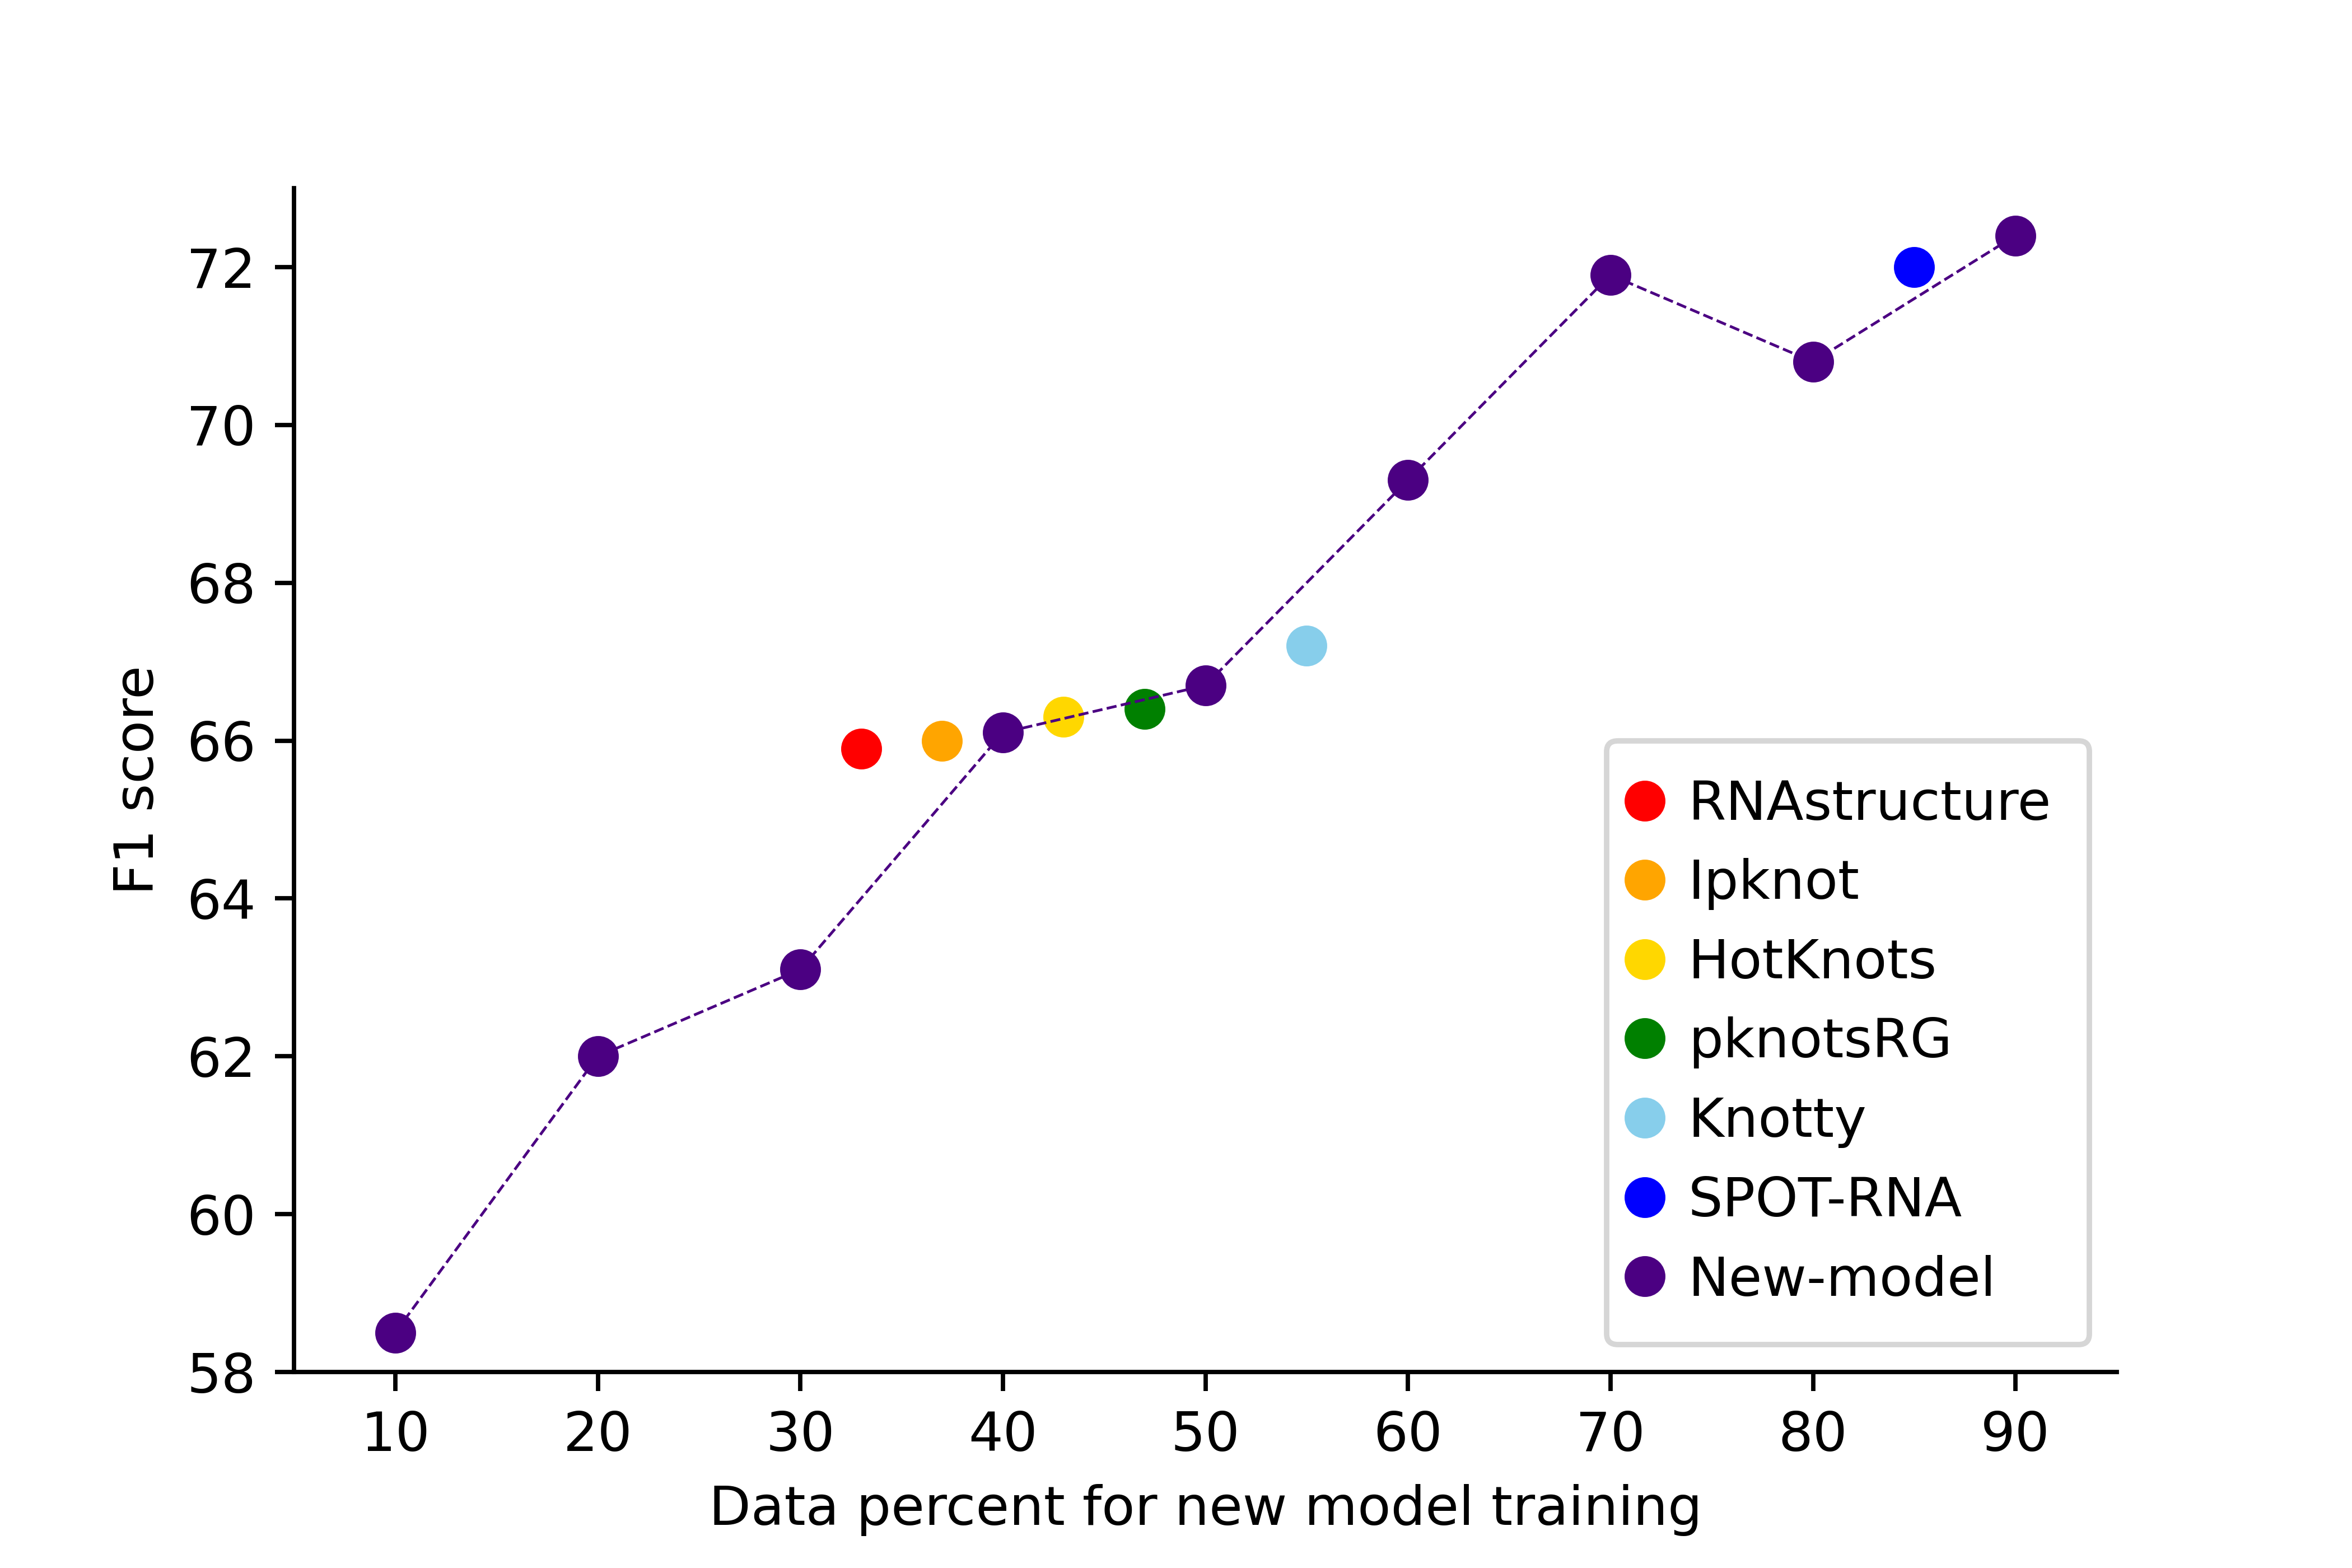
\includegraphics[width=10.5cm]{pics/plot_f1.png}
\end{frame}

\begin{frame}{Результаты}
Значения метрик $Precision$ и $Recall$ на тестовых выборках для нашей модели и на всей выборке для остальных инструментов

\centering
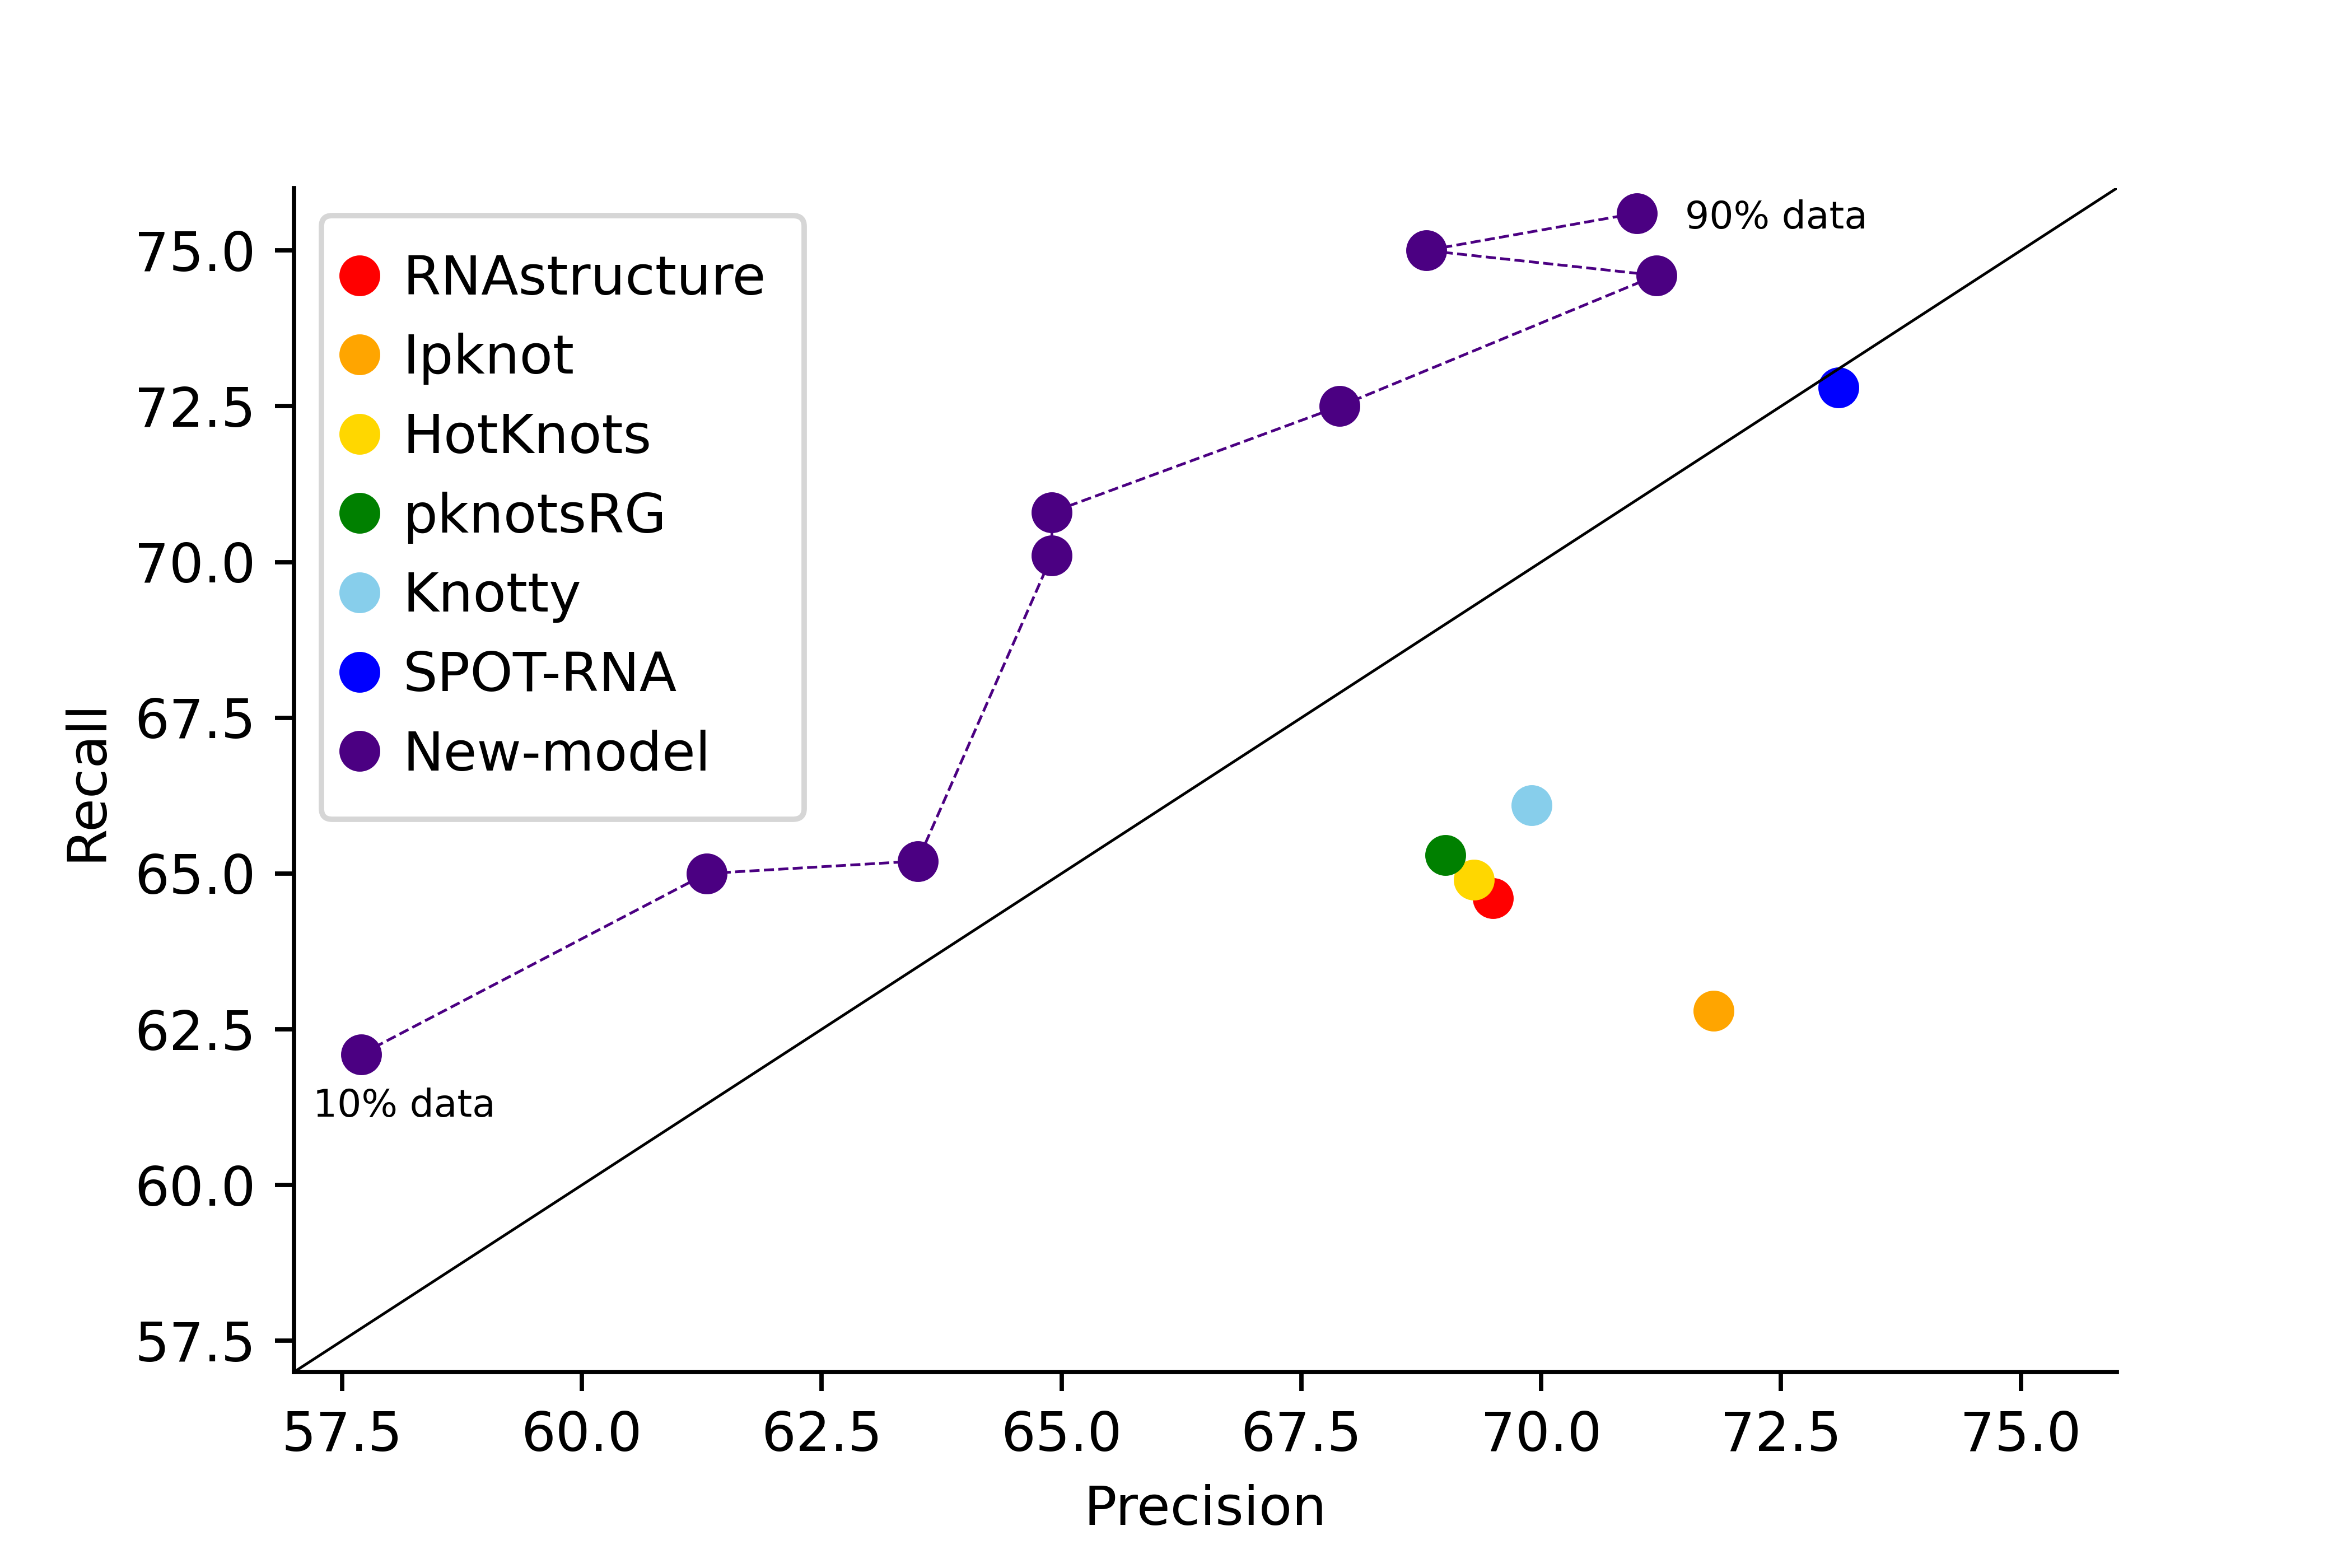
\includegraphics[width=10.5cm]{pics/plot_pr.png}
\end{frame}

\begin{frame}{Заключение}
\begin{itemize}
    \item Разработана архитектура решения для предсказания вторичной структуры РНК на основе комбинирования методов синтаксического анализа и машинного обучения
    \item Проведены эксперименты на реальных данных и сравнение полученных результатов с аналогами
    \item Представлен постер "Secondary structure prediction by combination of formal grammars and neural networks" на конференции Biata 2020 и опубликована одноименная статья (BMC Bioinformatics, Scopus)
\end{itemize}
\end{frame}

\newcommand{\backupbegin}{\setcounter{framenumber}{16}}
\newcommand{\backupend}{\setcounter{framenumber}{16}}
\appendix
\backupbegin
\begin{frame}{Время работы алгоритмов}
\begin{itemize}
    \item Операционная система: Ubuntu 20.04.2 LTS
    \item Центральный процессор: Intel Core i5-10210U CPU 1.60GHz
    \item Графический процессор: NVIDIA GeForce MX250
    \item Объем оперативной памяти: 7.5 GB
\end{itemize}
\begin{table}
\centering
\caption{Tools time performance on 100 sequences}
\ra{1.4}
\begin{tabular}{@{}lccc@{}}\toprule
& \multicolumn{2}{c}{\phantom{abc}  \phantom{abc}  \phantom{abc} Elapsed time, seconds}  \\
& Lengths 1-100 && Lengths 1-200  \\ \cmidrule{2-2} \cmidrule{4-4} 
Genegram & 28 && 39 \\
SPOT-RNA & 68 && 235 \\
Ipknot & 1 && 1 \\
Knotty & 283 && 3050 \\
RNAstructure & 10 && 15 \\
PknotsRG & 15 && 95 \\
HotKnots & 37 && 366 \\
\bottomrule
\end{tabular}
\label{table_time}
\end{table}
\end{frame}
\backupend
\end{document}